\documentclass{article}
\usepackage[utf8]{inputenc}
% \usepackage{fixltx2e}
\usepackage{hyperref}
\usepackage{amssymb,amsmath,amsthm}
\usepackage[makeroom]{cancel}

\usepackage{algorithm}
\usepackage[noend]{algpseudocode}

\usepackage{graphicx}


\title{q\textsubscript{IWAE}}

\author{Chris Cremer}
\date{January 2017}

\begin{document}

\maketitle


\begin{abstract}
This is an analysis of the implicit variational distribution defined by the IWAE ELBO \cite{burda2015importance}. I define the formula of the distribution, how to sample from it, and visualize intermediate distributions.
\end{abstract}





\section{Background}
The only difference between VAE and IWAE is their ELBOs. Although their variational distribution $q(z|x)$ is typically a Normal distribution, the multi-sample IWAE ELBO implicitly defines a variational distribution that differs from a Normal distribution. The following are the multi-sample equations for the log evidence (marginal likelihood), IWAE ELBO, and VAE ELBO, respectively. 
\begin{align} 
    log(p(x)) &=  log\left(E_{z_{1}...z_{k} \sim q(z|x)} \left[  \frac{1}{k}\sum_{i=1}^k \frac{p(x,z_i)}{q(z_i|x)}    \right]   \right)_{ML}
    \\
    & \geq E_{z_{1}...z_{k} \sim q(z|x)} \left[log\left(  \frac{1}{k}\sum_{i=1}^k \frac{p(x,z_i)}{q(z_i|x)}  \right)  \right]_{IWAE} \label{iwae_elbo}    \\
    & \geq E_{z_{1}...z_{k} \sim q(z|x)} \left[  \frac{1}{k}\sum_{i=1}^k log\left(\frac{p(x,z_i)}{q(z_i|x)}  \right)  \right]_{VAE} \label{vae_elbo}
\end{align}
VAE Gradient
\begin{align} 
    \nabla_{\Theta} \mathcal{L}_{VAE}(x) &= E_{z_{1}...z_{k} \sim q(z|x)} \left[ \frac{1}{k}  \sum_{i=1}^k  \nabla_{\Theta} log\left(\frac{p(x,z_i)}{q(z_i|x)}  \right)  \right] \label{vae_grad}
\end{align}
IWAE Gradient
\begin{align} 
    \nabla_{\Theta} \mathcal{L}_{IWAE}(x) &= E_{z_{1}...z_{k} \sim q(z|x)} \left[  \sum_{i=1}^k \tilde{w}_i \nabla_{\Theta} log\left(\frac{p(x,z_i)}{q(z_i|x)}  \right)  \right] \label{iwae_grad}
\end{align}
where $$\tilde{w}_i = \frac{\frac{p(x,z_i)}{q(z_i|x)}}{\sum_{j=1}^k \frac{p(x,z_j)}{q(z_j|x)}}$$
We see that the gradient of the VAE ELBO (\ref{vae_grad}) evenly weights the samples whereas the IWAE gradient (\ref{iwae_grad}) weights the samples based on their importance $\tilde{w}_i$.


% \begin{figure}[H]
%   \centering
%       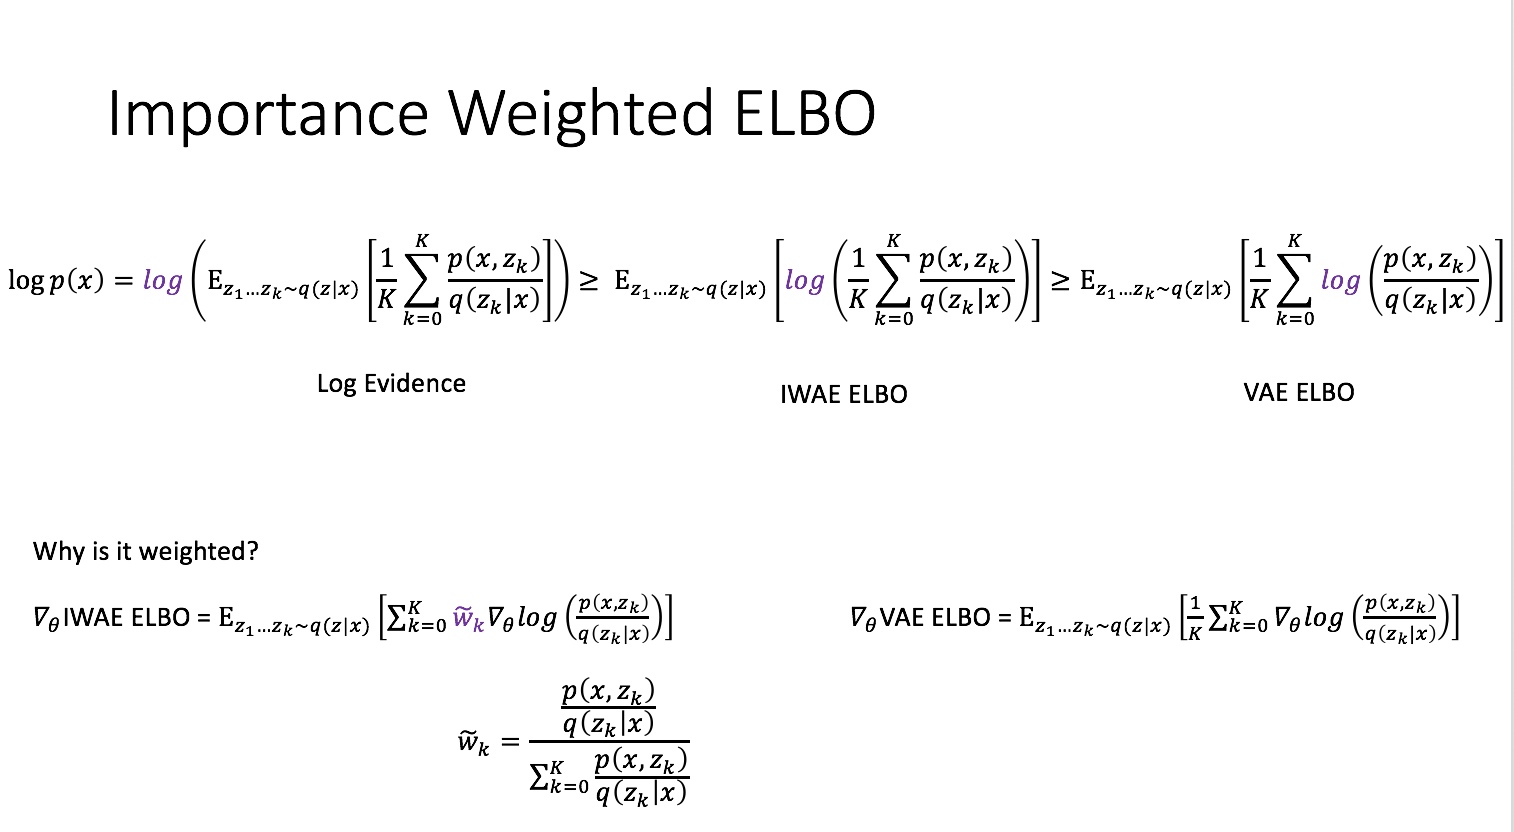
\includegraphics[width=1.\textwidth]{background.png}
%   \caption{Stuff to mention}
%   \label{background}
% \end{figure}









\section{q\textsubscript{IWAE} distribution}

The implicit variational distribution of the IWAE ELBO is a stochasticaly weighted version of the proposal/variational/posterior distribution $q(z|x)$:
\begin{align} 
    q_{IWAE}(z) &= k*E_{z_{1}...z_{k} \sim q(z|x)} \left[\frac{\frac{p(x,z)}{q(z|x)}}{\sum_{i=1}^k \frac{p(x,z_i)}{q(z_i|x)}}  \right] q(z|x) \\
    % &= E_{z_{1}...z_{k} \sim q(z|x)} \left[\frac{\frac{p(x,z)}{q(z|x)}}{\frac{1}{k}\sum_{i=1}^k \frac{p(x,z_i)}{q(z_i|x)}}  \right] q(z|x) \\
    &= E_{z_{1}...z_{k} \sim q(z|x)} \left[\frac{p(x,z)}{\frac{1}{k}\sum_{i=1}^k \frac{p(x,z_i)}{q(z_i|x)}}  \right]
    % &= \int_{z_{1}...z_{k}} \frac{q(z|x)p(x,z)}{\frac{1}{k}\sum_{i=1}^k \frac{p(x,z_i)}{q(z_i|x)}}  dz_1...z_k
\end{align}
% where the first sample is always z. *This might not be correct \\
\\
To confirm that this is the correct implicit q, we can plug it into the VAE ELBO (\ref{vae_elbo}) and see that it is equivalent to the IWAE ELBO (\ref{iwae_elbo}).
\begin{align} 
    log(p(x)) & \geq E_{z_{1}...z_{k} \sim q(z|x)} \left[  \frac{1}{k}\sum_{i=1}^k log\left(\frac{p(x,z_i)}{q_{IWAE}(z_i|x)}  \right)  \right] \\
    &= E_{z_{1}...z_{k} \sim q(z|x)} \left[  \frac{1}{k}\sum_{i=1}^k log\left(\frac{p(x,z_i)}{E_{z_{1}...z_{k} \sim q(z|x)} \left[\frac{p(x,z_i)}{\frac{1}{k}\sum_i^k \frac{p(x,z_j)}{q(z_j|x)}}  \right]}  \right)  \right] \label{with_e} \\
    &= E_{z_{1}...z_{k} \sim q(z|x)} \left[  \frac{1}{k}\sum_{i=1}^k log\left(\frac{p(x,z_i)}{\left(\frac{p(x,z_i)}{\frac{1}{k}\sum_j^k \frac{p(x,z_j)}{q(z_j|x)}}  \right)}  \right)  \right] \label{without_e} \\
    &= E_{z_{1}...z_{k} \sim q(z|x)} \left[  \frac{1}{k}\sum_{i=1}^k log\left(\frac{1}{k}\sum_{j=1}^k \frac{p(x,z_j)}{q(z_j|x)}  \right)  \right] \label{with_avg} \\
    &= E_{z_{1}...z_{k} \sim q(z|x)} \left[  log\left(\frac{1}{k}\sum_{j=1}^k \frac{p(x,z_j)}{q(z_j|x)}  \right)  \right] \label{without_avg}
\end{align}
Eqn. \ref{without_e} follows Eqn. \ref{with_e} since we are already taking the expectation over the samples. Eqn. \ref{without_avg} follows Eqn. \ref{with_avg} since nothing is indexed by i within the sum over indexes i. Now we can see that Eqn. \ref{without_avg} is equivalent to the IWAE ELBO (\ref{vae_elbo}).
% From Eqn. \ref{with_avg} to Eqn. \ref{without_avg}, we remove the outer average because there is already an average over the samples. 





\subsection{\texorpdfstring{$\boldsymbol{k=1}$}{k=1}} %
The first sample needs to be z. When $k=1$, the sample will be z, so
\begin{align} 
    q_{IWAE}(z) &= E_{z_{1} \sim q(z|x)} \left[\frac{\frac{p(x,z)}{q(z|x)}}{ \frac{p(x,z_1)}{q(z_1|x)}}  \right] q(z|x) \\
    &= E_{z_{1} \sim q(z|x)} \left[1  \right] q(z|x) \\
    % &= E_{z_{1} \sim q(z|x)} \left[\frac{p(x,z)}{\frac{1}{1}\sum_{i=1}^1 \frac{p(x,z_i)}{q(z_i|x)}}  \right] \\
    % &= \frac{p(x,z)}{ \frac{p(x,z)}{q(z|x)}}  \\
    &= q(z|x)
\end{align}
Since $q_{IWAE}(z)=q(z|x)$, it is equivalent to VAE when $k=1$, as expected.










\subsection{\texorpdfstring{$\boldsymbol{k=\infty}$}{k=inf}} %

Recall that the marginal likehood can be approximated by:
\begin{align} 
    p(x) &= E_{q(z|x)}\left[\frac{p(x,z)}{q(z|x)} \right] \approx \frac{1}{k}\sum_i^k \frac{p(x,z_i)}{q(z_i|x)}
\end{align}
where $z_i$ is sampled from $q(z_i|x)$. Thus, when $k=\infty$:
\begin{align} 
    q_{IWAE}(z) &= E_{z_{1}...z_{\infty} \sim q(z|x)} \left[\frac{p(x,z)}{E_{q(z|x)}\left[\frac{p(x,z)}{q(z|x)} \right]}  \right] \\
    &= \frac{p(x,z)}{p(x)} \\
    &= p(z|x)
\end{align}
Thus $q_{IWAE}(z)$ is equal to the truw posterior $p(z|x)$ when $k=\infty$, as expected.
% Remember that
% \begin{align} 
%     log(p(x)) = ELBO + KL(q(z|x)||p(z|x))
% \end{align}
% If k=$\infty$, $$q_{IWAE}(z)=p(z|x)$$ thus $$KL(q_{IWAE}(z)||p(z|x))=0$$ and $$p(x) = ELBO.$$
% The ELBO is tight.








% \subsection{Intermediate k: \texorpdfstring{$\boldsymbol{k<\infty}$}{k=int}}
% If $k<\infty$, then equation (\ref{eq:1}) becomes an approximation $\hat{p}(x)$ to the marginal likelihood $p(x)$. 
% \begin{align} 
%     q_{IWAE}(z) &= \frac{p(x,z)}{\hat{p}(x)} \\
%     &= \hat{p}(z|x)
% \end{align}
% Increasing the number of samples k, improves the approximation of the posterior distribution. 









\section{Sampling q\textsubscript{IWAE}}

The procedure to sample from $q_{IWAE}(z|x)$ is shown in Algo \ref{algo1}. It is equivalent to sampling-importance-resampling (SIR). \\
To visualize samples from $q(z|x)$ vs $q_{IWAE}$, I trained various networks on MNIST and displayed some reconstructions in Fig. \ref{recon}. 



\begin{algorithm}[H]
\caption{Sampling from the Importance Weighted posterior}\label{algo1}
\begin{algorithmic}[1]
    \State $N \gets \textit{number of draws}$
    \State $\textit{k} \gets \textit{number of samples}$
    \For {$i=0\textit{; } i<N\textit{; } i++$}
        \State $\textit{Draw k samples from}$ $q(z|x)$
        \State $\textit{Compute } \tilde{w} \textit{ for the k samples}$ where $\tilde w = w_i/\sum_{i=1}^{k} w_i$ and $w_i = \frac{p(x,z_i)}{q(z_i|x)}$
        \State $\textit{Draw an IW sample from } Cat(\tilde{w})$
    \EndFor
\end{algorithmic}
\end{algorithm}



\begin{figure}[H]
  \centering
      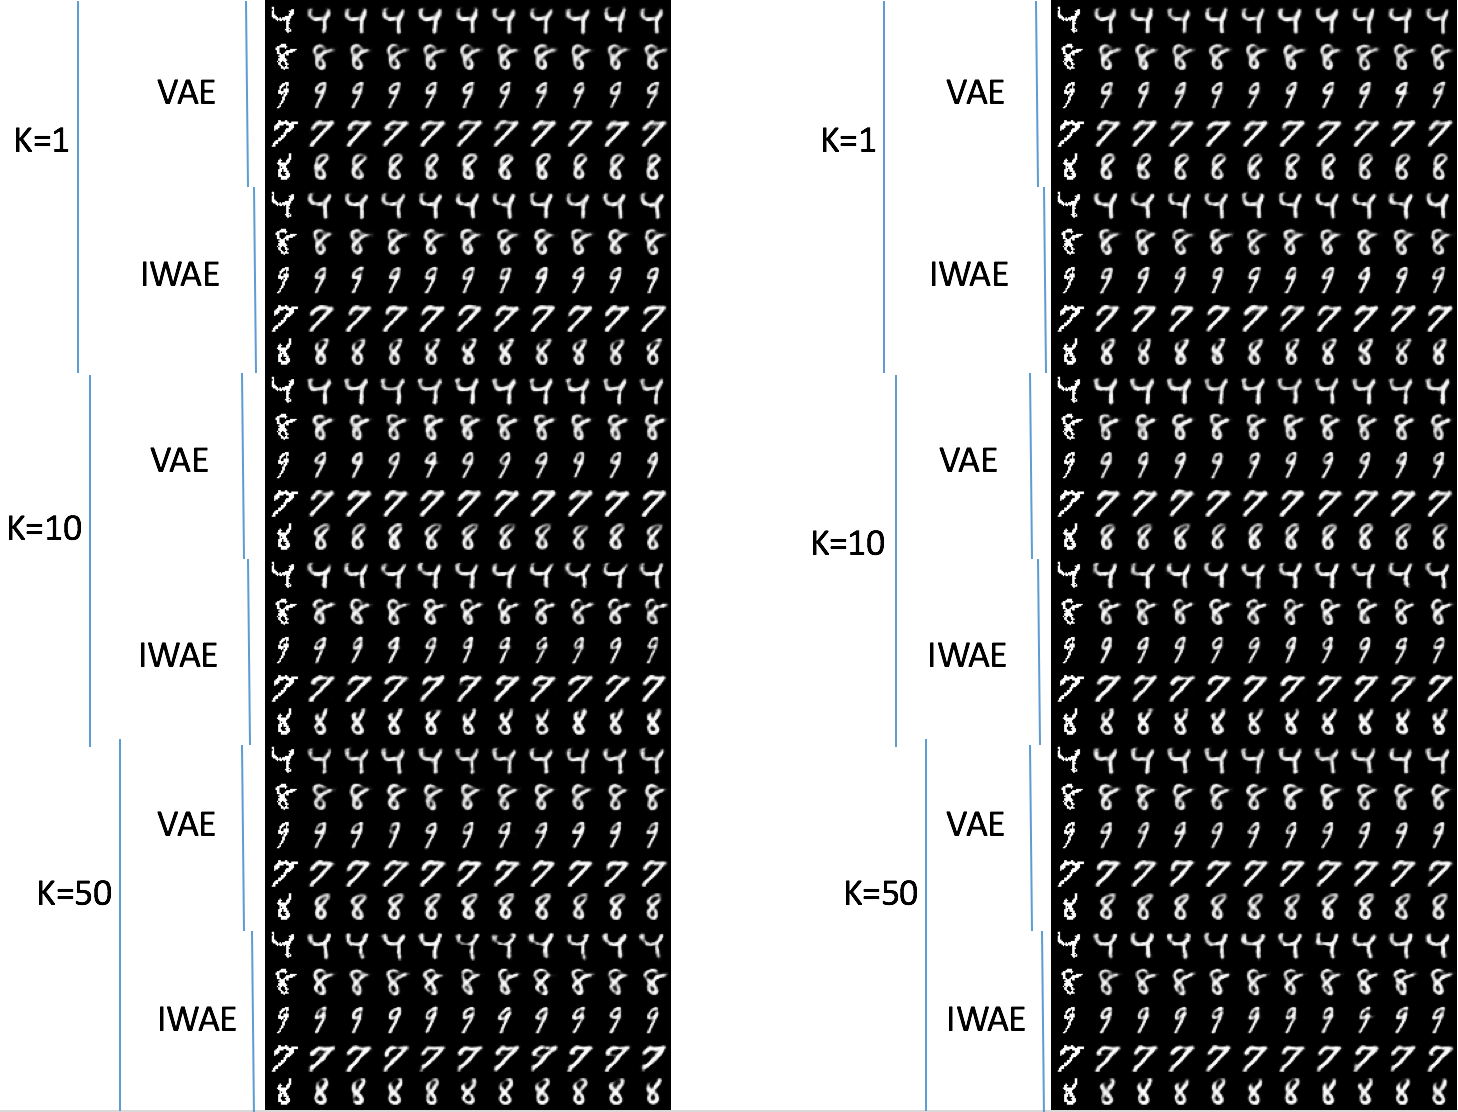
\includegraphics[width=1.\textwidth]{recons.png}
  \caption{Visualization of the reconstructions of samples from $q(z|x)$ (left) and $qIWAE$ (right). K indicates the number of samples and VAE/IWAE indicates the ELBO used during training. }
  \label{recon}
\end{figure}






\section{Visualizing q\textsubscript{IWAE}}

Now we can look at the intermediate variational distributions with different numbers of samples k. In Fig. \ref{viz} we see that as k increases, the approximate posterior approaches the true posterior. 

\begin{figure}[H]
  \centering
      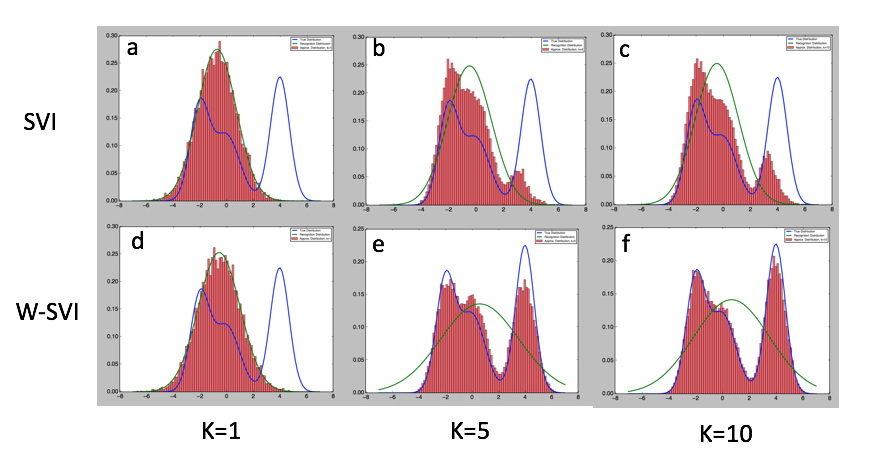
\includegraphics[width=1.\textwidth]{posteriors.png}
  \caption{Visualization of the importance weighted posterior. The blue distribution is the intractable distribution that we are trying to approximate. The green distribution is the variational distribution. The variational distributions of a, b, and c were optimized via SVI, whereas d, e, and f were optimized with a weighted SVI. The red histograms are weighted samples from the variational distribution.}
  \label{viz}
\end{figure}


















\section{Discussion}
The implicit q distribution defined by the IWAE ELBO is a stochastic approximation to the true posterior, which tightens the lower bound on the marginal likelihood.
% \\
% Other stuff\\
% - not sure if the q iwae is correct. should the 1/k be there. and missing sum? \\
% - remmeber what the reason I couldnt cancel out the term in the q iwae thing i did before. \\




% - FIrst think is k=1 i think is wrong because expectation would make it 1, not q(z|x)

% % add vizualiztion. 
% \begin{equation} \label{eq1}
% \begin{split}
%     log(p(x)) &\geq E_{z_1...z_k\sim q(z|x)}\left[\frac{1}{k} \sum_{i=0}^{k} log \left(   \frac{p(x,z_i)}{q(z_i|x)} \right) \right]
% \end{split}
% \end{equation}



% probably describe where the formula comes from. ie using the iwae elbo\\
% maybe have a background section on the elbo , iwae elbo, and the q distribution .


% also could show that iwae elbo at inf is a tight bound so KL must be 0, um is that true. 
% logp(x) = iwae elbo with k=inf, right so KL must be 0, meaning the approximate is equal to posterior. 
% So just need to show how it goes to p(x,z). but im having a hard time doing that .

% $\frac{1}{k}\sum_i^k \frac{p(x,z_i)}{q(z_i|x)}$ is an unbiased estimator of $E_{q(z|x)}\left[\frac{p(x,z)}{q(z|x)} \right]$

% p(x) is the marginal likelihood

% $Z_p$ is the marginal likelihood p(x). !!!! not the partiiton funciotn since were integrating over z. 
% Show the elbo is 0 when this is true. 


% \begin{align} 
%     q_{IWAE}(z) &= E_{z_{1}...z_{k} \sim q(z|x)} \left[ \tilde{w} \right] q(z|x)\\
%     &= E_{z_{1}...z_{k} \sim q(z|x)} \left[\frac{\frac{p(x,z)}{q(z|x)}}{\frac{p(x,z)}{q(z|x)} + \sum_i^k \frac{p(x,z_i)}{q(z_i|x)}}  \right] q(z|x)  \\
%     &= E_{z_{1}...z_{k} \sim q(z|x)} \left[\frac{p(x,z)}{\frac{p(x,z)}{q(z|x)} + \sum_i^k \frac{p(x,z_i)}{q(z_i|x)}}  \right]
% \end{align}

% I remember there being a reason I couldn't do eqn (3) \\
% This equation is definitely wrong. that sum goes to inf, making w=0. 

% \begin{align} 
%     q_{IWAE}(z) &= E_{z_{1}...z_{k} \sim q(z|x)} \left[\frac{\frac{p(x,z)}{q(z|x)}}{\frac{p(x,z)}{q(z|x)} + \cancel{\sum_i^k \frac{p(x,z_i)}{q(z_i|x)}}  }  \right] q(z|x)  \\
%     &= q(z|x)
% \end{align}

% E_{z_{1}...z_{k} \sim q(z|x)} \left[ \tilde{w} \right] q(z|x)\\
%     &= E_{z_{1}...z_{k} \sim q(z|x)} \left[\frac{w}{\sum_{i=1}^k w_i} \right] q(z|x)\\


    % &= E_{z_{1}...z_{k} \sim q(z|x)} \left[\frac{\frac{p(x,z)}{q(z|x)}}{\frac{p(x,z)}{q(z|x)} + \cancel{\sum_i^k \frac{p(x,z_i)}{q(z_i|x)}}  }  \right] q(z|x)  \\


% % davids
% \begin{align} 
%     q_{IWAE}(z) &= E_{z_{1}...z_{k} \sim q(z|x)} \left[ \sum_k \left( \frac{\frac{p(x,z_k)}{q(z_k|x)}}{\sum_i^k \frac{p(x,z_i)}{q(z_i|x)}}  \right) \right] q(z|x)
% \end{align}
% Maybe I understood it wrong, this is from a picture I took. 

% \begin{align} 
%     q_{IWAE}(z) &= E_{z_{1} \sim q(z|x)} \left[\frac{p(x,z)}{ \frac{p(x,z)}{q(z|x)}}  \right] \\
%     &= q(z|x)
% \end{align}

% E_{z_{1}...z_{k} \sim q(z|x)} \left[\frac{p(x,z)}{p(x)}  \right] \\
%     % &= \left(\frac{\frac{p(x,z)}{q(z|x)}}{p(x)}  \right) q(z|x)  \\


% \newpage

\bibliographystyle{ieeetr}
\bibliography{refs.bib}



\end{document}




